\hypertarget{organizational-project-skill-demand}{%
\section{Organizational Project Skill
Demand}\label{organizational-project-skill-demand}}

Question: How many organizations are using this project and could hire
me if I become proficient?

\hypertarget{description}{%
\subsection{Description}\label{description}}

Organizations engage with open source projects through use and
dependencies. This metric is aimed at determining downstream demand of
skills related to an open source project. This metric looks at
organizations that deploy a project as part of an IT infrastructure,
other open source projects with declared dependencies, and references to
the project through social media, conference mentions, blog posts, and
similar activities.

\hypertarget{objectives}{%
\subsection{Objectives}\label{objectives}}

As a developer, I'd like to invest my skills and time in a project that
has a likelihood of getting me a decent paying job in the future. People
can use the Downstream Organizational Impact of a Project Software
metric to discover which projects are used by organizations, and they
may, therefore, be able to pursue job opportunities with, possibly
requiring IT support services.

\hypertarget{implementation}{%
\subsection{Implementation}\label{implementation}}

Base metrics include:

\begin{itemize}
\tightlist
\item
  Number of organizations that created issues for a project
\item
  Number of organizations that created pull requests for a project
\item
  Number of organizations that blog or tweet about a project
\item
  Number of organizations that mention a project in open hiring requests
\item
  Number of organizations that are represented at meetups about this
  project
\item
  Number of other projects that are dependent on a project
\item
  Number of books about a project
\item
  Google search trends for a project
\end{itemize}

\hypertarget{visualizations}{%
\subsubsection{Visualizations}\label{visualizations}}

The following visualization demonstrates the number of downstream
projects dependendent on the project in question. While this
visualization does not capture the entirety of the Downstream
Organizational Impact of a Project Software metric, it provides a visual
for a portion.

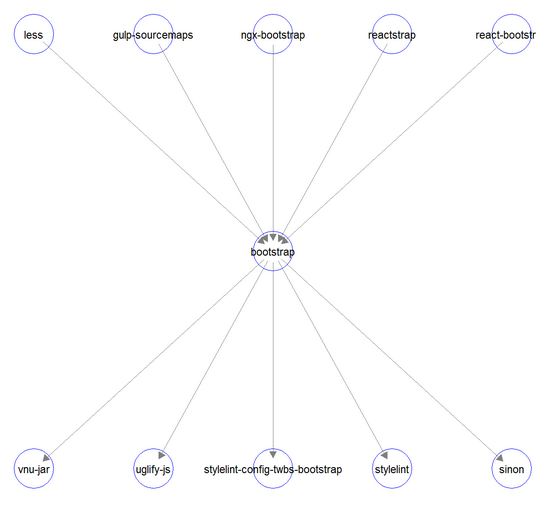
\includegraphics{images/organizational-project-skill-demand_paper.png}

Other visualizations could include Google search trends (React vs.
Angular vs. Vue.js)

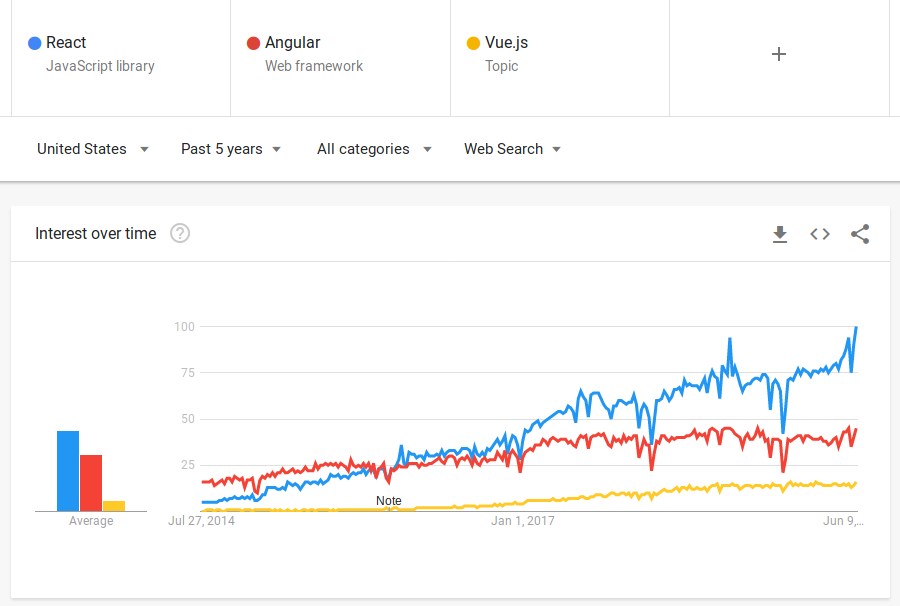
\includegraphics{images/organizational-project-skill-demand_google-trends.png}

ThoughtWorks publishes a series called 'Tech Radar' that shows the
popularity of technologies.

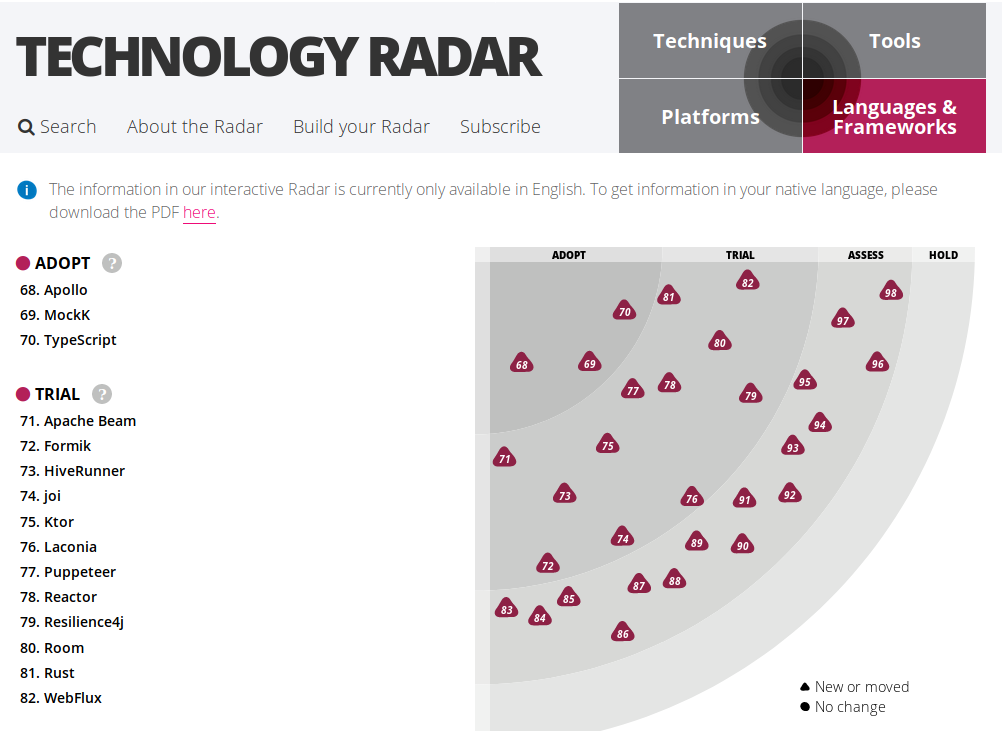
\includegraphics{images/organizational-project-skill-demand_tech-radar.png}

Tech Radar allows you to drill down on projects to see how the
assessment has changed over time.

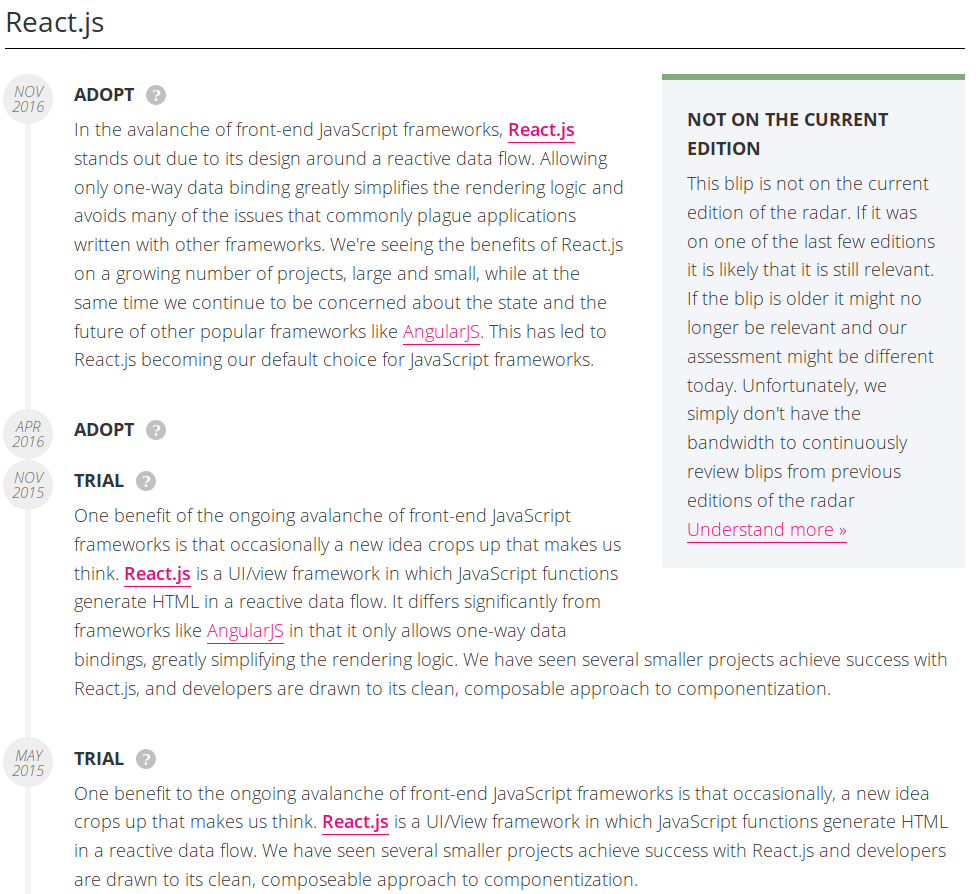
\includegraphics{images/organizational-project-skill-demand_tech-react.png}

StackOverview publishes an annual developer's survey

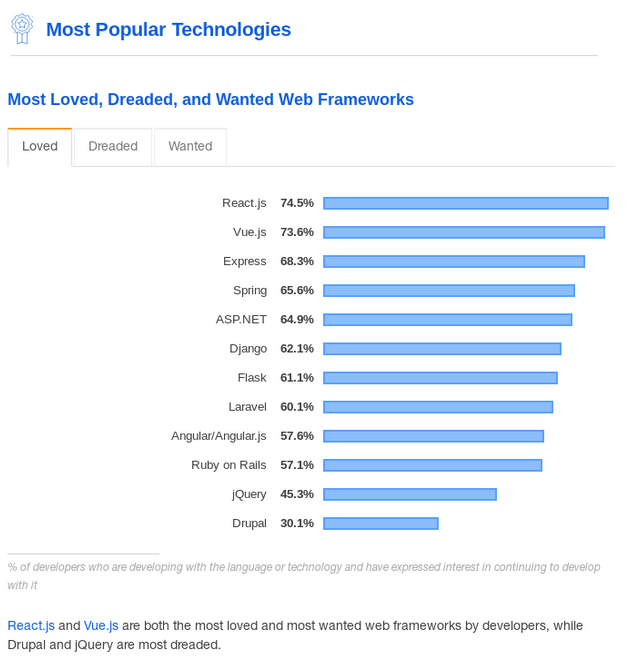
\includegraphics{images/organizational-project-skill-demand_stack-overflow.png}

\hypertarget{tools-providing-the-metric}{%
\subsubsection{Tools Providing the
Metric}\label{tools-providing-the-metric}}

\begin{itemize}
\tightlist
\item
  Google Trends - for showing search interest over time
\item
  ThoughtWorks TechRadar - project assessments from a tech consultancy
\item
  StackOverflow Developer's Survey - annual project rankings
\item
  Augur; Examples are available for multiple repositories:

  \begin{itemize}
  \tightlist
  \item
    \href{http://augur.osshealth.io/repo/Rails\%20(wg-value)/rails/overview}{Rails}
  \item
    \href{http://augur.osshealth.io/repo/Zephyr-RTOS/zephyr/overview}{Zephyr}
  \item
    \href{http://augur.osshealth.io/repo/Apache\%20(wg-value)/cloudstack/overview}{CloudStack}
  \end{itemize}
\end{itemize}

\hypertarget{references}{%
\subsection{References}\label{references}}

\begin{itemize}
\tightlist
\item
  \href{https://opensource.org/sponsors}{Open Source Sponsors}
\item
  \href{https://opensource.com/article/19/1/fiscal-sponsors-open-source}{Fiscal
  Sponsors and Open Source}
\item
  \href{https://www.networkworld.com/article/2867020/big-names-like-google-dominate-open-source-funding.html}{Large
  Corporate OpenSource Sponsors}
\item
  \href{https://www.npmjs.com/package/google-trends-api}{Google Trends
  API}
\item
  \href{https://aisel.aisnet.org/cgi/viewcontent.cgi?article=1496\&context=amcis2018}{Measuring
  Open Source Software Impact}
\item
  \href{https://www.thoughtworks.com/radar}{ThoughtWorks Tech Radar}
\item
  \href{https://insights.stackoverflow.com/survey/2019\#technology}{Stack
  Overflow Developer's Survey}
\end{itemize}
